\documentclass[border=4pt]{standalone}
\usepackage{fontspec}
\usepackage{amsmath}
\usepackage{unicode-math}
\setmainfont{Latin Modern Roman}
\setmathfont{Latin Modern Math}
\usepackage{pgfplots}
\usepackage{pgfplotstable}
\pgfplotsset{compat=1.18}
\usepackage{tkz-euclide}
\usetikzlibrary{arrows.meta,calc,angles,quotes,patterns,3d,backgrounds}
\definecolor{ink}{HTML}{123428}
\definecolor{asy}{HTML}{475569}
\definecolor{mint}{HTML}{86e0bd}
\tikzset{asym/.style={asy, line width=0.9pt, dash pattern=on 5pt off 3.5pt},
         guide/.style={gray!70, line width=0.6pt, densely dotted},
         dot/.style={circle, inner sep=0pt, minimum size=5pt, draw=white, line width=0.5pt},
         odot/.style={circle, inner sep=0pt, minimum size=5.5pt, fill=white, line width=1pt},
         lab/.style={font=\footnotesize, inner sep=1.5pt, text=ink}}
\begin{document}
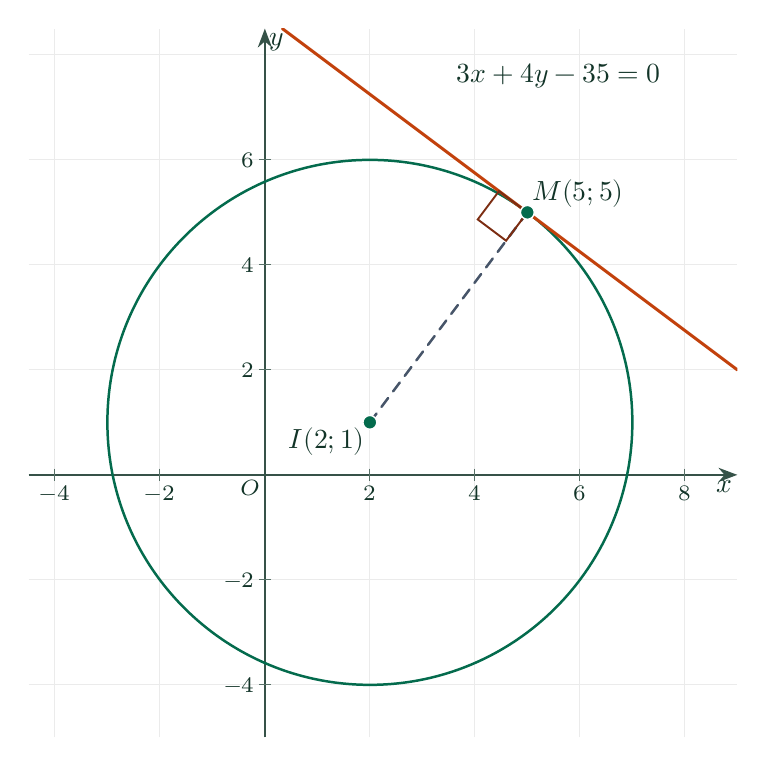
\begin{tikzpicture}[x=0.6667cm, y=0.6667cm]
\draw[gray!16, line width=0.4pt] (-4,-5) -- (-4,8.5) (-2,-5) -- (-2,8.5) (0,-5) -- (0,8.5) (2,-5) -- (2,8.5) (4,-5) -- (4,8.5) (6,-5) -- (6,8.5) (8,-5) -- (8,8.5);
\draw[gray!16, line width=0.4pt] (-4.5,-4) -- (9,-4) (-4.5,-2) -- (9,-2) (-4.5,0) -- (9,0) (-4.5,2) -- (9,2) (-4.5,4) -- (9,4) (-4.5,6) -- (9,6) (-4.5,8) -- (9,8);
\draw[ink!85, line width=0.7pt, -{Stealth[length=2.4mm]}] (-4.5,0) -- (9,0) node[anchor=north east, lab, font=\normalsize] {$x$};
\draw[ink!85, line width=0.7pt, -{Stealth[length=2.4mm]}] (0,-5) -- (0,8.5) node[anchor=north west, lab, font=\normalsize] {$y$};
\draw[ink!70] (-4,0.12000000000000001) -- (-4,-0.12000000000000001) node[below, lab, font=\footnotesize] {$-4$};
\draw[ink!70] (-2,0.12000000000000001) -- (-2,-0.12000000000000001) node[below, lab, font=\footnotesize] {$-2$};
\draw[ink!70] (2,0.12000000000000001) -- (2,-0.12000000000000001) node[below, lab, font=\footnotesize] {$2$};
\draw[ink!70] (4,0.12000000000000001) -- (4,-0.12000000000000001) node[below, lab, font=\footnotesize] {$4$};
\draw[ink!70] (6,0.12000000000000001) -- (6,-0.12000000000000001) node[below, lab, font=\footnotesize] {$6$};
\draw[ink!70] (8,0.12000000000000001) -- (8,-0.12000000000000001) node[below, lab, font=\footnotesize] {$8$};
\draw[ink!70] (0.12000000000000001,-4) -- (-0.12000000000000001,-4) node[left, lab, font=\footnotesize] {$-4$};
\draw[ink!70] (0.12000000000000001,-2) -- (-0.12000000000000001,-2) node[left, lab, font=\footnotesize] {$-2$};
\draw[ink!70] (0.12000000000000001,2) -- (-0.12000000000000001,2) node[left, lab, font=\footnotesize] {$2$};
\draw[ink!70] (0.12000000000000001,4) -- (-0.12000000000000001,4) node[left, lab, font=\footnotesize] {$4$};
\draw[ink!70] (0.12000000000000001,6) -- (-0.12000000000000001,6) node[left, lab, font=\footnotesize] {$6$};
\node[lab, anchor=north east] at (0,0) {$O$};
\tkzDefPoint(2,1){I}
\tkzDefPoint(5,5){M}
\tkzDefPoint(7,1){tmp1}
\tkzDefPoint(9,2){tmp2}
\tkzDefPoint(0.333333,8.5){tmp3}
\tkzDefPoint(0.333333,8.5){tmp4}
\begin{scope}
\clip (-4.5,-5) rectangle (9,8.5);
\tkzDrawCircle[draw={rgb,255:red,4;green,107;blue,77}, line width=0.9pt](I,tmp1)
\tkzDrawSegment[draw={rgb,255:red,71;green,85;blue,105}, line width=0.90pt, dash pattern=on 4pt off 3pt](I,M)
\tkzDrawSegment[draw={rgb,255:red,194;green,65;blue,12}, line width=1.08pt](tmp2,tmp3)
\end{scope}
\tkzMarkRightAngle[size=0.45, draw={rgb,255:red,124;green,45;blue,18}, line width=0.7pt](I,M,tmp4)
\node[dot, fill={rgb,255:red,4;green,107;blue,77}] at (I) {};
\node[dot, fill={rgb,255:red,4;green,107;blue,77}] at (M) {};
\node[lab, font=\normalsize] at (5.6,7.6) {$3x + 4y - 35 = 0$};
\node[lab, font=\normalsize, anchor=north east] at (2,1) {$I(2; 1)$};
\node[lab, font=\normalsize, anchor=south west] at (5,5) {$M(5; 5)$};
\end{tikzpicture}
\end{document}
